% arara: xelatex: {synctex: true}
% arara: indent: {overwrite: yes}
\documentclass[]{IMTexam}

\usepackage[enums]{IMTtikz}

\givecredits
\author{Isabella B.}
\USPN{11810773}
\date{}
\lecture{Física I} % disciplina
\lcode{4302111}
\hwtype{Resolução} % o que é
\examname{Lista 8} % prova

\begin{document}

\maketitle

\begin{questions}

	\question Considere a colisão completamente inelástica entre dois corpos de massas $ m_1 $ e $ m_2 $. Para tempos $ t < 0 $ os dois corpos estão em movimento em direções ortogonais, até chegar ao tempo $ t = 0 $ em que eles colidem. Descreva o movimento dos corpos para tempos $ t > 0 $, ou seja, depois da colisão.

	\begin{solution}

	\end{solution}

	\question O universo é composto por cerca de 70\% de energia escura (responsável pela expansão acelerada do universo) enquanto o restante 30\% pode-se dividir entre um 5\% de matéria ordinária (prótons, elétrons etc) e um 25\% de matéria escura, matéria que interage gravitacionalmente mas que ou não interage eletromagneticamente ou interage muito fracamente. Existem experimentos na Terra (por exemplo, Xenon1T ou DarkSide) que procuram as colisões entre matéria escura e núcleos do detector. Considere a colisão elástica entre uma partícula de matéria escura e um núcleo:

	\begin{parts}
		\part Trabalhando no referencial inercial de repouso do núcleo (ou seja, onde o núcleo está parado), calcule a velocidade da partícula de matéria escura depois da colisão sabendo que a velocidade típica das partículas de matéria escura que chegam na Terra é da ordem de $ v \simeq \num{1e-3}c $, onde $ c $ é a velocidade da luz. Suponha inicialmente que a colisão aconteça em uma dimensão e que todas as partículas envolvidas (inclusive o núcleo) possam se movimentar livremente;

		\begin{solution}

		\end{solution}

		\part Repita o cálculo do item (a) considerando agora uma colisão em três dimensões. é possível expressar a velocidade final da matéria escura apenas em termos de $ v $ e das massas da matéria escura e do núcleo?

		\begin{solution}

		\end{solution}

		\part Calcule a energia cinética de recuo do núcleo em termos das quantidades relevantes;

		\begin{solution}

		\end{solution}

		\part O que pode ser dito em relação à velocidade da matéria escura depois da colisão no caso $ m_{\text{DM}} \ll m_{\text{núcleo}} $?

		\begin{solution}

		\end{solution}

		\part Os experimentos acima mencionados conseguem detectar experimentalmente apenas energias de recuo do núcleo $ E_{\text{recuo}} \gtrsim \SI{1}{\kilo\electronvolt} $. É verdade que matéria escura com massa qualquer pode dar origem a uma colisão detectável experimentalmente? Considere a colisão como sendo unidimensional, a massa do núcleo da ordem de \SI{100}{\giga\electronvolt} e tome o limite $ m_{\text{DM}} \ll m_{\text{núcleo}} $ para simplificar o cálculo.

		\begin{solution}

		\end{solution}
	\end{parts}

	\question O pêndulo balístico é um dispositivo onde um bloco de massa $ M $, preso por um haste de massa desprezível, pode girar livremente, sem atrito, em torno de um ponto fixo $ O $. O dispositivo é usado para determinar a velocidade de impacto de projéteis, que vão parar dentro do bloco. Determine a velocidade de um projétil que colide com o bloco em função da altura na qual o bloco para depois da colisão.

	\begin{solution}

	\end{solution}

	\question Considere a colisão elástica de um corpo com uma parede em movimento. Qual a velocidade final do corpo no caso em que \begin{romanlistinline}[label=(\roman*)]
		\item a parede está em movimento na mesma direção e sentido do corpo, e
		\item a parede está em movimento na mesma direção mas sentido oposto ao corpo.
	\end{romanlistinline}

	\begin{solution}

	\end{solution}

	\question Suponha que uma pessoa de massa $ M $ pule de uma altura $ h $ sem movimento horizontal. Suponha também que, quando a pessoa colide com o chão, o centro de massa da pessoa se movimenta para baixo de uma distância $ s $. Determine:

	\begin{parts}
		\part a força média durante a colisão, supondo que essa tem duração $ \Delta t $;

		\begin{solution}
			Sendo a velocidade terminal de uma pessoa que pula de uma altura $ h $ sob a ação da gravidade $ g $
			\begin{equation}\label{eq:fspeedt}
				v=\sqrt{2g\,h},
			\end{equation}
			pela relação do impulso, temos
			\begin{align}
				\int_{0}^{\Delta t}F\dif t & =\Delta p\nonumber                                  \\
				F_{m}\,\Delta t            & =M\del{v-0}\nonumber                                \\
				F_m                        & =\dfrac{M\sqrt{2g\,h}}{\Delta t}.\label{eq:Fmfall1}
			\end{align}
		\end{solution}

		\part supondo uniforme a força que o chão exerce na pessoa (e portanto a aceleração), escreva a força média em termos de $ s $;

		\begin{solution}
			Como a pessoa percorre $ 2s $ durante a queda, temos
			\begin{equation}\label{eq:Dtfall}
				\Delta t=\dfrac{2s}{v}
			\end{equation}
			de tal forma que, pela segunda lei de Newton
			\begin{align}
				F_m & =M\,a_m\nonumber                                          \\
				F_m & =M\dfrac{\Delta v}{\Delta t}\nonumber                     \\
				\intertext{substituindo \ref{eq:fspeedt} e \ref{eq:Dtfall}, temos}
				F_m & =M\dfrac{2g\,h}{2s}=M\,g\dfrac{h}{s}.\label{eq:hsrelfall}
			\end{align}
		\end{solution}

		\part interprete os resultados achados de acordo com a seguinte pergunta: ``durante uma queda, por quê é melhor se agachar o quanto mais possível para reduzir a força do impacto?''

		\begin{solution}
			De \ref{eq:hsrelfall} sabemos que, quanto maior deslocamento na queda, menor a força média exercida pelo chão na pessoa.

			Dessa forma, a melhor coisa a se fazer numa queda é agachar-se.
		\end{solution}

		\part Suponha que seu professor (de massa $ M \simeq \SI{70}{\kilo\gram} $) pule de uma altura de \SI{1}{\meter}, tentando não quebrar o tornozelo. A força que o tornozelo consegue sustentar sem quebrar é da ordem de \SIrange{4}{8}{\kilo\newton} (dependendo da idade). Quanto vale a distância $ s $ que garante que o tornozelo não quebre?

		\begin{solution}
			Aproximando $ g=\SI{10}{\meter\per\second\squared} $, e considerando a força média máxima suportada \SI{4}{\kilo\newton}, temos, por \ref{eq:hsrelfall}
			\[ s=M\,g\dfrac{h}{F_m}=\dfrac{\num{70}\cdot\num{10}\cdot1}{\num{4000}}= \SI{0.175}{\meter}. \]
		\end{solution}
	\end{parts}

	\question \label{ques:q6}Uma estrela em equilíbrio é uma estrela para a qual a pressão gravitacional (que tenderia a causar o colapso) é balanceada pela pressão gerada pelas reações nucleares que acontecem no seu interior. A situação de equilíbrio é sustentada enquanto há combustível nuclear. Quando a pressão das reações nucleares não é mais suficiente para sustentar a  pressão gravitacional, a estrela colapsa e, surpreendentemente, dá origem à explosão de uma supernova. Para entender a física envolvida, vamos modelar as partes externas da estrela como uma bola de massa $ M_1 $, enquanto que o caroço interno será modelado como uma bola de massa $ M_2\ll M_1 $. A situação é mostrada na Fig. \ref{fig:fig1}. Vamos supor, por simplicidade, que a altura inicial seja $ h $ para as duas bolas (ignoramos os tamanhos), e que a velocidade inicial dos dois corpos seja nula. Calcule a altura final de $ M_1 $ supondo que, em primeira aproximação, todas as colisões sejam elásticas. Como você pode usar esse modelo simples para entender a explosão da supernova? (dica: qual o referencial melhor para descrever a colisão entre $ M_1 $ e $ M_2 $ que acontece depois que $ M_2 $ ja colidiu com o chão?).

	\begin{figure}[H]
		\centering
		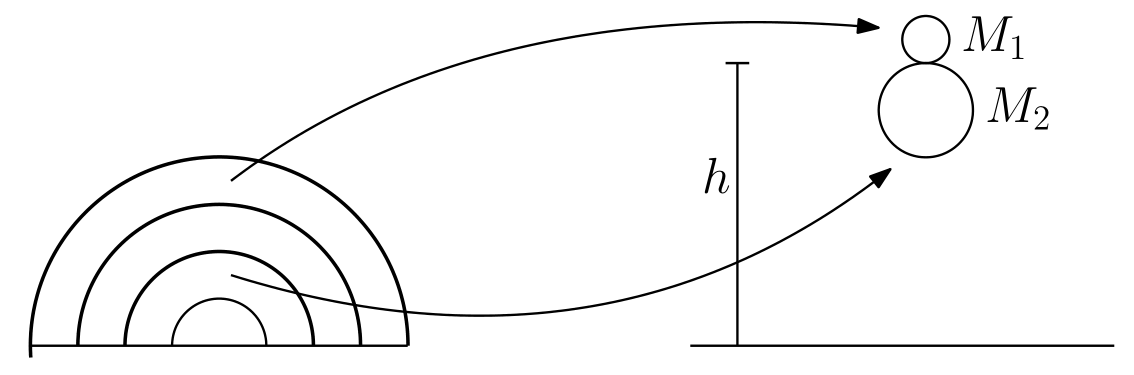
\includegraphics[width=0.7\linewidth]{fig1}
		\caption{As partes da estrela do exercício \ref{ques:q6} podem ser modeladas como duas bolas, de massas $ M_1 \ll M_2, $ em queda sob a ação da gravidade.}
		\label{fig:fig1}
	\end{figure}

	\begin{solution}

	\end{solution}

	\question Considere a colisão elástica entre um corpo em movimento com velocidade $ v $ e um corpo parado com a mesma massa. Mostre que é sempre verdade que, depois da colisão, o ângulo entre as velocidades dos dois corpos é \ang{90}.

	\begin{solution}

	\end{solution}

	\question O fenômeno de \textit{gravitational slingshot} (estilingue gravitacional) consiste em utilizar o movimento de um planeta de massa $ M $ para modificar --- geralmente aumentando --- a velocidade de uma sonda espacial de massa $ m \ll M $ que está se movimentando na direção do planeta. Para simplificar, suponha que os movimentos da sonda e do planeta aconteçam no mesmo eixo.

	\begin{parts}
		\part Convença-se que, dado que estamos interessados nas velocidades da sonda antes e depois do encontro com o planeta, podemos descrever o processo como uma colisão, ignorando os detalhes da atração gravitacional entre os dois corpos;

		\begin{solution}

		\end{solution}

		\part Dado o item precedente, identifique qual entre os problemas desta lista descreve uma física parecida. Use-o como inspiração para calcular a velocidade final da sonda.

		\begin{solution}

		\end{solution}
	\end{parts}

	\question Vimos em aula que várias estrelas estão orbitando o centro da Via Láctea, um local conhecido como \textit{Sagittarius A$ ^{\star} $}. Uma delas, chamada de S2, tem uma órbita elíptica de grande excentricidade, cujo eixo semi-maior é $ R=\SI{970}{\astronomicalunit} $, onde usamos unidades astronômicas, em que $ \SI{1}{\astronomicalunit}=\SI{1.5e11}{\meter} $ é a distância média da Terra ao Sol. Observações dessa estrela ao longo de mais de uma década indicam que a órbita de S2 possui um período de aproximadamente 16 anos.

	\begin{parts}
		\part Apenas utilizando a 3ª Lei de Kepler, estime a massa do objeto em \textit{Sagittarius A$ ^{\star} $} em unidades da massa do Sol.

		\begin{solution}

		\end{solution}

		\part Agora faça um cálculo usando a Lei da Gravitação Universal de Newton.
		Você pode fazer aproximações com respeito ao movimento de S2. Compare o seu resultado com o resultado do item (a). As duas respostas conferem? Justifique.

		\begin{solution}

		\end{solution}
	\end{parts}

	\question Considere um sistema planetário com uma estrela sendo orbitada por um único planeta.

	\begin{parts}
		\part Tente demonstrar que, se o planeta executa uma órbita circular, então a estrela também deve seguir uma órbita circular.

		\begin{solution}

		\end{solution}

		\part Mostre que nesse caso ambos de fato orbitam o centro de massa desse sistema, e que esse fato nem sequer depende da natureza da força gravitacional --- basta que a força entre os dois objetos seja uma força central.

		\begin{solution}

		\end{solution}
	\end{parts}

\end{questions}
\end{document}
